\documentclass[12pt,oneside,noprintercorrection]{iut}

% Inclusion des packages nécessaires
\usepackage{macros}

\usepackage[utf8]{inputenc}
\usepackage[T1]{fontenc}
\usepackage[french]{babel}
\usepackage{graphicx}
\usepackage{amsmath}
\usepackage{hyperref}
\usepackage{xcolor}
\usepackage{array}
\usepackage{multirow}
\usepackage{booktabs}
\usepackage{float}
\usepackage{tikz}
\usetikzlibrary{positioning, shapes.geometric, arrows.meta, calc, decorations.pathreplacing}
\usepackage{pgfplots}
\pgfplotsset{compat=1.18}

% Toutes les images produites par l'application sont dans img_use/
\graphicspath{{img_use/}}

% Couleurs utilisées dans les schémas et les encadrés
\definecolor{bleudoux}{RGB}{74, 127, 165}
\definecolor{vertdoux}{RGB}{74, 140, 74}
\definecolor{rougedoux}{RGB}{176, 58, 58}
\definecolor{orangedoux}{RGB}{222, 145, 51}

\NoChapterHead

% Encadré pour mettre en avant une idée clé ou une distinction importante
\newcommand{\encadre}[2]{%
  \par\medskip\noindent
  \begin{center}
  \fcolorbox{bleudoux}{bleudoux!6}{%
    \begin{minipage}{0.93\linewidth}
      \vspace{1mm}
      \textbf{\textcolor{bleudoux}{#1}}\\[1mm]
      #2
      \vspace{1mm}
    \end{minipage}}
  \end{center}\par\medskip}

% Informations de la page de titre
\ThesisTitle{Assurance Prévision}
\ThesisKind{Introduction aux Data Sciences}
\ThesisPresentedThe{écrit le 25 mai 2026}
\ThesisAuthor{Bruno HANNA et Amal DEROUICH}
\LogoLaboOuEntreprise{img/LogoEntreprise.pdf}
\EncadrantUniv = {Audrey FONGUE et David DUPONT}

\begin{document}

% Page de titre
\MakeThesisTitlePage
\tableofcontents
\mainmatter

% ══════════════════════════════════════════════════════════════════════════════
\SpecialSection{Introduction}
% ══════════════════════════════════════════════════════════════════════════════

Le métier de l'assurance repose sur une question simple à formuler mais difficile à
trancher. Ce client va-t-il, oui ou non, coûter de l'argent à l'assureur ? Derrière
chaque contrat, il y a une estimation du risque, et plus elle est juste, mieux
l'entreprise fixe ses tarifs et anticipe ses dépenses. Longtemps affaire de jugement
d'expert, ce travail peut aujourd'hui être confié à un programme qui apprend lui-même,
à partir d'exemples passés, à reconnaître les profils à risque.
\newline
\newline
C'est l'objet de ce projet. On dispose d'un fichier décrivant dix mille conducteurs dont
on sait, pour chacun, s'il a déclaré un sinistre. À partir de ces données, on cherche à
prédire si un nouveau conducteur en déclarera un à son tour. En science des données, on
parle de \textbf{classification supervisée binaire}, supervisée parce qu'on apprend sur
des exemples dont la réponse est déjà connue, et binaire parce que cette réponse ne prend
que deux valeurs.
\newline
\newline
La variable à prédire, \texttt{outcome}, vaut \texttt{0} en l'absence de sinistre et
\texttt{1} sinon. Les autres colonnes (âge, expérience de conduite, revenu, type de
véhicule, nombre d'infractions…) sont les indices sur lesquels le programme fonde sa
décision. Un point pèsera sur toute la suite. Les deux réponses ne sont pas également
fréquentes, puisque environ deux conducteurs sur trois n'ont pas de sinistre contre un
sur trois qui en a un ; on parle de \textbf{classes déséquilibrées}, et ce déséquilibre
changera la façon d'interpréter les résultats.
\newline
\newline
Au-delà du résultat chiffré, l'intérêt est de parcourir la démarche complète d'une étude
de données, que résume la figure~\ref{fig:pipeline}. On comprend d'abord les données, on
les nettoie et on les met en forme, on sépare ce qui sert à apprendre de ce qui sert à
juger, on entraîne un modèle, on l'évalue, on le compare à d'autres et l'on conserve le
meilleur. Chaque chapitre correspond à l'une de ces étapes.

\begin{figure}[H]
  \centering
  \resizebox{\linewidth}{!}{%
  \begin{tikzpicture}[
    >={Stealth[length=2.6mm]},
    etape/.style={rectangle, rounded corners=3pt, draw=bleudoux, line width=0.6pt,
                  fill=bleudoux!8, align=center, minimum height=1.35cm, text width=2.5cm},
    fleche/.style={->, line width=0.7pt, draw=gray}]
    \node[etape] (a) {Comprendre\\les données};
    \node[etape, right=7mm of a] (b) {Nettoyer\\et préparer};
    \node[etape, right=7mm of b] (c) {Séparer\\apprentissage\\et test};
    \node[etape, right=7mm of c] (d) {Entraîner\\un modèle};
    \node[etape, right=7mm of d] (e) {Évaluer\\la qualité};
    \node[etape, right=7mm of e] (f) {Comparer\\et conserver\\le meilleur};
    \draw[fleche] (a) -- (b);
    \draw[fleche] (b) -- (c);
    \draw[fleche] (c) -- (d);
    \draw[fleche] (d) -- (e);
    \draw[fleche] (e) -- (f);
  \end{tikzpicture}}
  \caption{Les grandes étapes du projet.}
  \label{fig:pipeline}
\end{figure}

\medskip
\noindent\textbf{Note sur les figures.} Les graphiques chiffrés (histogrammes, cartes de
corrélation, courbes de performance) sont directement produits par l'application
développée pour ce projet. Les schémas explicatifs, eux, ont été dessinés
spécifiquement pour ce rapport afin de rendre les concepts plus intuitifs.

% ══════════════════════════════════════════════════════════════════════════════
\chapter{Comprendre les données avant de les utiliser}
% ══════════════════════════════════════════════════════════════════════════════

Avant d'entraîner le moindre modèle, il faut prendre le temps de regarder les
données telles qu'elles sont. Cette étape est souvent négligée par impatience, alors
qu'elle conditionne tout le reste, car un modèle n'est jamais meilleur que les données
qu'on lui fournit. L'objectif ici est donc modeste mais essentiel. Il faut savoir
combien de données on a, de quelle nature elles sont, et dans quel état.

\section{Ce que contient le jeu de données}

Le fichier rassemble dix mille conducteurs décrits par dix-huit colonnes. L'une d'elles,
\texttt{id}, n'est qu'un numéro d'identification qui ne dit rien sur le risque et sera
écartée. Une autre, \texttt{outcome}, est la réponse que l'on cherche à prédire. Restent
seize colonnes qui décrivent le conducteur et son véhicule, et qui serviront d'indices.
\newline
\newline
Toutes ces colonnes ne se ressemblent pas, et c'est un point qu'il faut bien saisir car
il revient sans cesse par la suite. On distingue trois grandes natures de variables :

\begin{itemize}
  \item Les \textbf{variables continues}, qui peuvent prendre une infinité de valeurs sur
        une échelle, comme le kilométrage annuel ou le score de crédit.
  \item Les \textbf{variables de comptage}, qui dénombrent des événements comme le nombre
        d'infractions pour excès de vitesse, le nombre d'accidents passés ou le nombre de
        condamnations pour conduite en état d'ivresse.
  \item Les \textbf{variables catégorielles}, qui désignent une appartenance à un groupe,
        comme le sexe, le type de véhicule, la tranche d'âge ou le niveau d'études. Certaines de
        ces catégories sont d'ailleurs stockées sous forme de texte dans le fichier
        d'origine.
\end{itemize}

\encadre{Une distinction à garder en tête}{Une même opération de nettoyage peut
être parfaitement justifiée sur une variable continue et complètement absurde sur une
variable catégorielle. Confondre les deux natures conduit à abîmer les données sans s'en
rendre compte. Garder cette distinction en tête est la clé de toute l'étape de
préparation décrite au chapitre suivant.}

\section{Les distributions, ou la forme des données}

Regarder un tableau de chiffres ne dit pas grand-chose ; visualiser la \emph{forme} de
chaque variable est bien plus parlant. La figure~\ref{fig:histogrammes} montre, pour
chaque variable, comment se répartissent les conducteurs, en distinguant par une couleur
ceux qui ont eu un sinistre de ceux qui n'en ont pas eu. Cette superposition est
précieuse, car lorsqu'une variable sépare nettement les deux couleurs, c'est le signe
qu'elle contient une information utile pour la prédiction.

\begin{figure}[H]
  \centering
  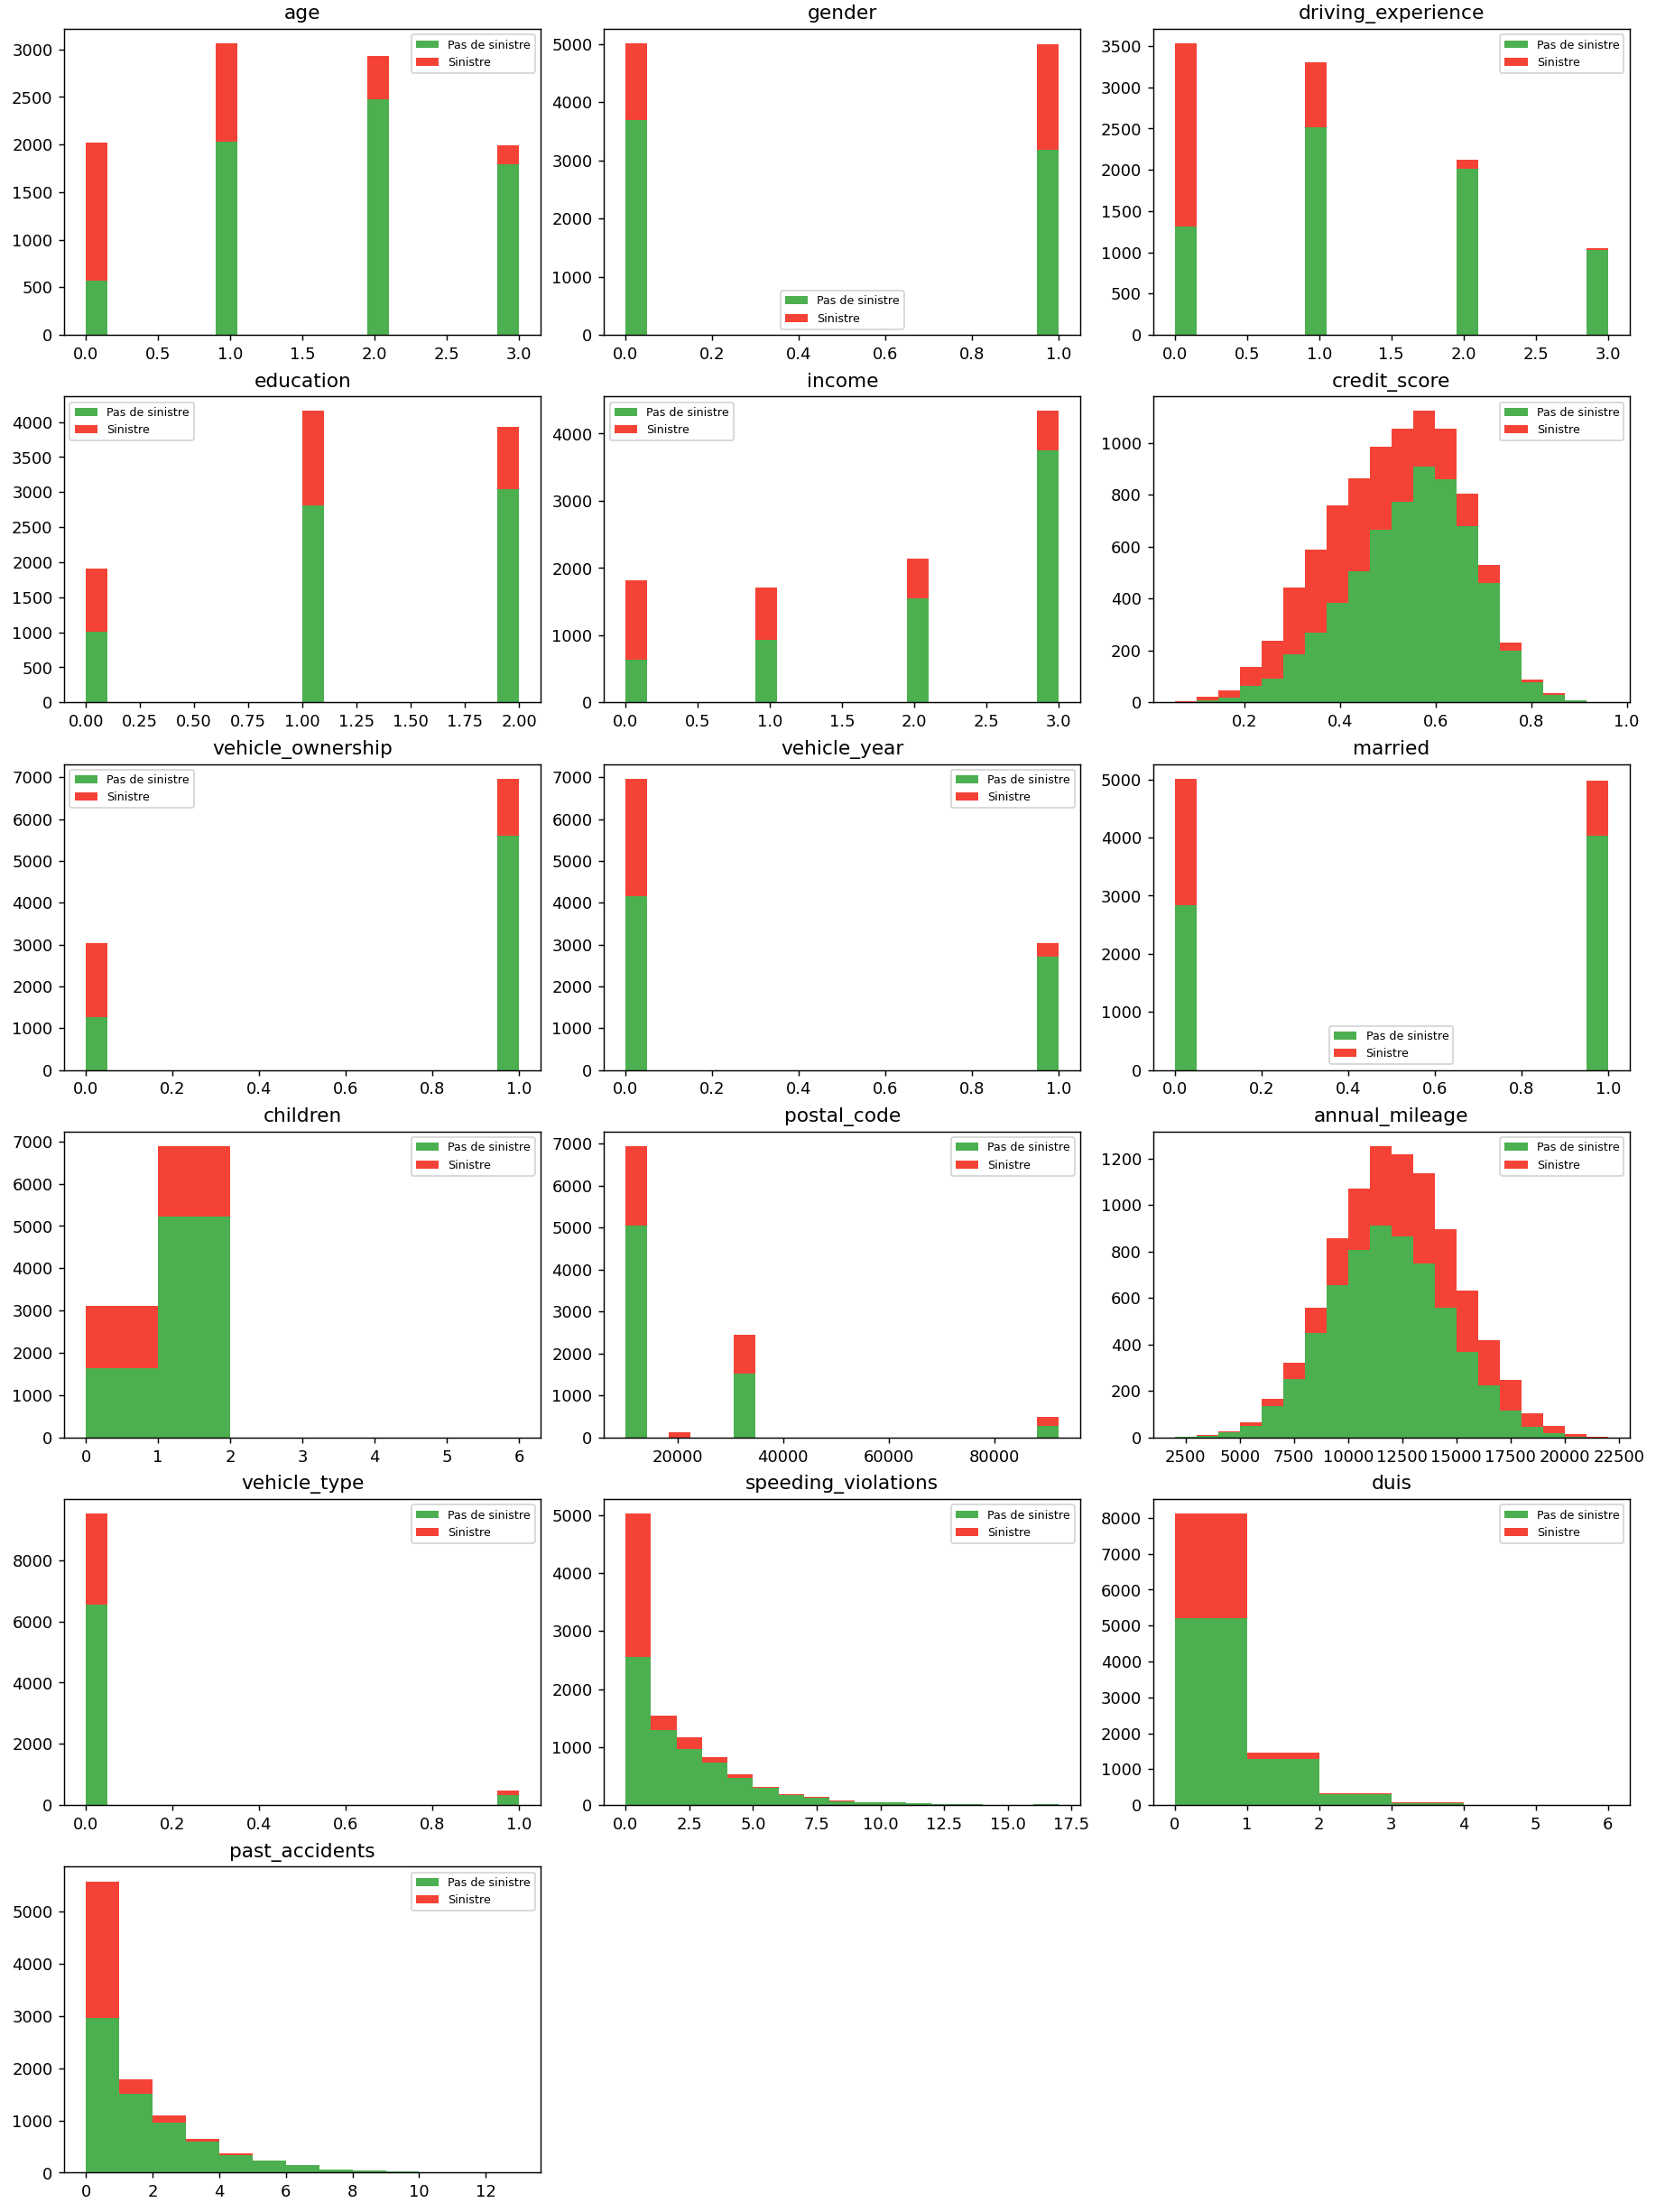
\includegraphics[width=0.85\linewidth]{histogrammes.png}
  \caption{Répartition de chaque variable selon la présence d'un sinistre.}
  \label{fig:histogrammes}
\end{figure}

On remarque au passage que plusieurs variables de comptage sont autour de zéro, par
exemple la grande majorité des conducteurs n'ayant aucune condamnation pour conduite en
état d'ivresse. Cette particularité sera importante au moment du nettoyage.

\section{Deux défauts de qualité à corriger}

En inspectant les données, deux problèmes de qualité apparaissent, qu'il faudra traiter
avant de modéliser.
\newline
\newline
Le premier est celui des \textbf{valeurs manquantes}, des cases restées vides faute d'avoir
été renseignées. Seules deux colonnes sont concernées, le score de crédit (environ
982 valeurs absentes, soit près de 10~\%) et le kilométrage annuel (environ 957,
également près de 10~\%). Cela reste limité, à peine un dixième des valeurs de ces deux
colonnes. La règle de bon sens veut que l'on ne supprime des lignes que lorsque les
trous sont massifs (au-delà d'un tiers, typiquement) ; ici, mieux vaut combler les vides
plutôt que de jeter des conducteurs entiers.
\newline
\newline
Le second problème est celui des \textbf{valeurs aberrantes}, des valeurs si éloignées
des autres qu'elles en paraissent suspectes, comme un kilométrage démesuré. La
figure~\ref{fig:aberrants} en donne un aperçu sous forme de boîtes à moustaches, un
type de graphique conçu exactement pour cela, expliqué au chapitre
suivant. Ces valeurs extrêmes se concentrent sur le score de crédit, le kilométrage, et
les comptages d'infractions et d'accidents.

\begin{figure}[H]
  \centering
  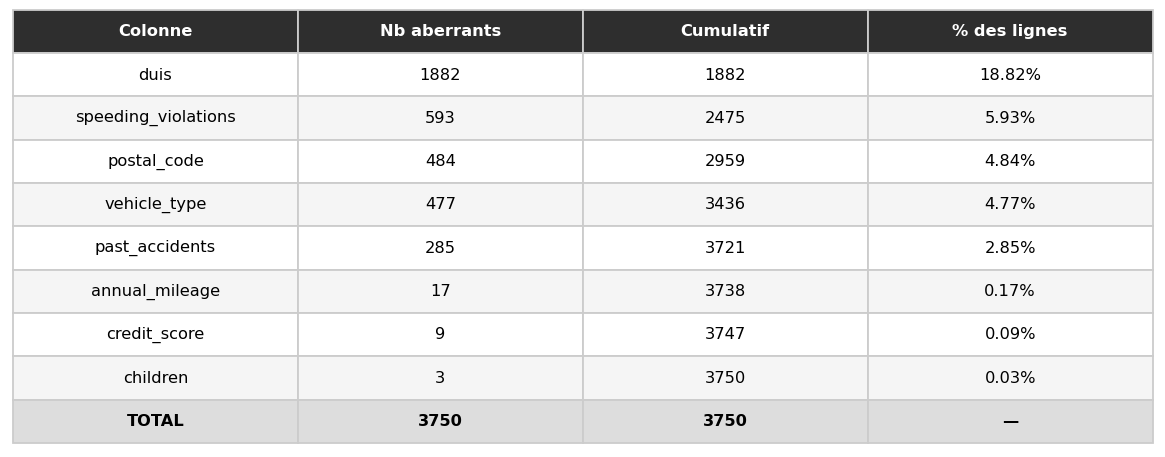
\includegraphics[width=0.88\linewidth]{aberrants.png}
  \caption{Boîtes à moustaches des principales variables.}
  \label{fig:aberrants}
\end{figure}

Comprendre ces deux défauts, c'est déjà savoir ce qu'il faudra réparer. C'est tout
l'objet du chapitre suivant.

% ══════════════════════════════════════════════════════════════════════════════
\chapter{Préparer les données}
% ══════════════════════════════════════════════════════════════════════════════

\section{Pourquoi ne peut-on pas travailler sur les données brutes ?}

On pourrait être tenté de donner les données telles quelles au modèle et de le laisser
se débrouiller. Ce serait une erreur. Un algorithme d'apprentissage est, au fond, une
machine à repérer des régularités, et elle prend les données très au sérieux, jusque dans
leurs défauts. Si on lui présente des cases vides, des valeurs absurdes ou des unités
incohérentes, il apprendra ces défauts aussi fidèlement que les vraies tendances. C'est
le principe bien connu en informatique selon lequel des déchets en entrée ne peuvent
donner que des déchets en sortie. La qualité de ce qui sort ne dépasse jamais celle de
ce qui entre.

\begin{figure}[H]
  \centering
  \begin{tikzpicture}[
    >={Stealth[length=2.8mm]},
    boite/.style={rectangle, rounded corners=3pt, draw, line width=0.6pt,
                  align=center, minimum height=1.5cm, text width=3.2cm},
    fleche/.style={->, line width=0.9pt}]
    % chemin du haut : données sales -> modèle -> mauvaises prédictions
    \node[boite, fill=rougedoux!10, draw=rougedoux] (sale) {Données\\non préparées\\{\small(trous, valeurs absurdes,\\échelles incohérentes)}};
    \node[boite, fill=gray!10, right=12mm of sale] (m1) {Apprentissage\\du modèle};
    \node[boite, fill=rougedoux!10, draw=rougedoux, right=12mm of m1] (mauvais) {Prédictions\\peu fiables};
    \draw[fleche, draw=rougedoux] (sale) -- (m1);
    \draw[fleche, draw=rougedoux] (m1) -- (mauvais);
    % chemin du bas : données propres -> modèle -> bonnes prédictions
    \node[boite, fill=vertdoux!10, draw=vertdoux, below=10mm of sale] (propre) {Données\\préparées\\{\small(complètes, cohérentes,\\à la même échelle)}};
    \node[boite, fill=gray!10, right=12mm of propre] (m2) {Apprentissage\\du modèle};
    \node[boite, fill=vertdoux!12, draw=vertdoux, right=12mm of m2] (bon) {Prédictions\\fiables};
    \draw[fleche, draw=vertdoux] (propre) -- (m2);
    \draw[fleche, draw=vertdoux] (m2) -- (bon);
  \end{tikzpicture}
  \caption{Déchets en entrée, déchets en sortie.}
  \label{fig:gigo}
\end{figure}

La préparation poursuit donc un objectif clair, illustré par la figure~\ref{fig:gigo}.
Il s'agit de transformer un tableau imparfait en un jeu de données entièrement numérique,
sans trou, sans valeur extravagante, et dont toutes les colonnes parlent la même langue.
Cela se fait en quatre gestes, détaillés ci-dessous.

\section{Combler les valeurs manquantes}

La première idée qui vient à l'esprit pour combler un trou est d'y mettre une valeur
typique de la colonne. Mais laquelle ? On hésite généralement entre deux candidates,
la \textbf{moyenne} et la \textbf{médiane}. La différence entre les deux est subtile mais
importante. La moyenne additionne toutes les valeurs et divise par leur nombre ; elle est
donc sensible aux extrêmes, qu'une seule valeur démesurée suffit à tirer vers le haut. La
médiane, elle, est simplement la valeur du milieu lorsqu'on range les conducteurs par
ordre croissant ; quelques valeurs extrêmes ne la déplacent presque pas.

\encadre{Moyenne ou médiane ?}{Dans un quartier où tout le monde gagne un salaire
modeste sauf un milliardaire, la moyenne des revenus est élevée et trompeuse, alors que
la médiane reste représentative de l'habitant ordinaire. C'est pourquoi les trous des
variables numériques sont comblés par la \emph{médiane}, qui résiste aux valeurs extrêmes
encore non traitées à ce stade.}

Pour les variables catégorielles, ni l'une ni l'autre n'a de sens (quelle serait la
moyenne d'un type de véhicule ?). On y met alors la \textbf{valeur la plus
fréquente}, appelée le mode, ce qui revient à faire le pari le plus probable.

\section{Maîtriser les valeurs aberrantes}

Pour repérer les valeurs aberrantes, on s'appuie sur la notion d'\textbf{écart
interquartile}, qui est aussi ce que résume la boîte à moustaches vue plus haut. L'idée
est de regarder où se situe le gros de la troupe. On note $Q_1$ la valeur en dessous de
laquelle se trouvent les 25~\% les plus bas, et $Q_3$ celle en dessous de laquelle se
trouvent les 75~\% les plus bas. Entre les deux s'étend la moitié centrale des
conducteurs, et l'on considère comme atypique toute valeur qui s'éloigne trop de cette
zone. La figure~\ref{fig:iqr} montre cette anatomie.

\begin{figure}[H]
  \centering
  \begin{tikzpicture}[font=\small]
    % axe
    \draw[->, gray] (-0.3,0) -- (12.6,0) node[right, black]{valeur};
    % moustaches
    \draw[line width=0.8pt] (2,1.4) -- (4,1.4); % gauche
    \draw[line width=0.8pt] (2,1.05) -- (2,1.75);
    \draw[line width=0.8pt] (7,1.4) -- (9,1.4); % droite
    \draw[line width=0.8pt] (9,1.05) -- (9,1.75);
    % boite Q1..Q3
    \draw[line width=0.9pt, fill=bleudoux!15] (4,0.8) rectangle (7,2.0);
    \draw[line width=1.1pt] (5.3,0.8) -- (5.3,2.0); % médiane
    % outliers
    \fill[rougedoux] (10.4,1.4) circle (2.6pt);
    \fill[rougedoux] (11.4,1.4) circle (2.6pt);
    % étiquettes hautes
    \node[above] at (4,2.05) {$Q_1$};
    \node[above] at (5.3,2.05) {médiane};
    \node[above] at (7,2.05) {$Q_3$};
    \node[align=center, above, text=rougedoux] at (10.9,1.7) {valeurs\\atypiques};
    % étiquettes basses (bornes)
    \draw[densely dotted, gray] (2,0)--(2,1.05);
    \draw[densely dotted, gray] (9,0)--(9,1.05);
    \node[below, align=center, text width=2.6cm] at (2,-0.05) {borne basse\\{\scriptsize$Q_1-1{,}5\,$IQR}};
    \node[below, align=center, text width=2.6cm] at (9,-0.05) {borne haute\\{\scriptsize$Q_3+1{,}5\,$IQR}};
    % accolade IQR
    \draw[decorate, decoration={brace, amplitude=5pt}, gray] (4,2.7) -- (7,2.7)
        node[midway, above=4pt]{\footnotesize IQR (moitié centrale)};
  \end{tikzpicture}
  \caption{Anatomie d'une boîte à moustaches.}
  \label{fig:iqr}
\end{figure}

Reste à décider quoi faire de ces valeurs atypiques. Les supprimer serait excessif, car une
valeur extrême n'est pas forcément fausse, et un conducteur multipliant les infractions
est justement le plus intéressant à étudier pour un assureur. On a donc choisi de
les \textbf{écrêter}, c'est-à-dire que plutôt que de jeter la valeur, on la ramène à la
borne la plus proche. La différence entre supprimer et écrêter est essentielle. La
suppression fait disparaître l'information, tandis que l'écrêtage la conserve tout en
limitant son influence excessive.

\encadre{Adapter le nettoyage à chaque colonne}{Appliquer une recette de nettoyage
aveuglément à toutes les colonnes est dangereux. Sur une variable de comptage très
tassée sur zéro, la règle de l'écart interquartile peut conclure que toute valeur non
nulle est atypique et tout écraser à zéro, faisant disparaître une variable entière.
On a donc adapté le traitement à la \emph{nature} de chaque colonne, sans aucun
écrêtage sur les catégories, avec un écrêtage doux sur les comptages, et l'écrêtage classique
sur les variables continues. La même opération peut soigner une colonne et en détruire
une autre ; il faut donc choisir au cas par cas.}

\section{Traduire le texte en nombres avec l'encodage}

Un algorithme ne sait manipuler que des nombres. Or cinq colonnes sont stockées sous
forme de texte (l'expérience de conduite, le niveau d'études, le revenu, l'ancienneté du
véhicule et son type). Il faut donc les traduire en entiers. C'est l'étape qui a demandé
le plus de réflexion, et elle illustre bien comment un choix en apparence technique peut
fausser tout un modèle.
\newline
\newline
La méthode la plus immédiate consiste à laisser un outil tout-fait attribuer un numéro à
chaque catégorie. Le problème est que cet outil ne connaît pas le \emph{sens} des
catégories, qu'il numérote simplement dans l'ordre alphabétique.

\encadre{Le piège de l'ordre alphabétique}{Pour le niveau d'études, l'ordre alphabétique
donnerait \texttt{high school}~$=0$, \texttt{none}~$=1$, \texttt{university}~$=2$.
Autrement dit, l'absence de diplôme se retrouverait \emph{entre} le lycée et l'université,
ce qui n'a aucun sens. Pour le revenu, on obtiendrait un classement tout aussi
fantaisiste. Comme le modèle utilisé est linéaire, c'est-à-dire qu'il
suppose qu'une valeur plus grande pousse régulièrement la prédiction dans un sens, un
ordre incohérent brouille complètement la relation entre la variable et le risque.}

Il faut ici distinguer deux familles de variables catégorielles, car elles n'appellent
pas le même traitement. Une variable est \textbf{ordinale} lorsque ses catégories ont un
ordre naturel, un niveau d'études allant clairement du plus bas au plus haut. Elle est
\textbf{nominale} lorsque ses catégories ne se classent pas, aucune raison ne permettant
de dire qu'un type de véhicule est supérieur à un autre. Pour ces variables, l'ordre a
un sens ; il a donc été fixé à la main, dans l'ordre logique, du moins
au plus d'expérience, du diplôme le plus bas au plus élevé, du revenu le plus faible au
plus fort. Le modèle reçoit ainsi des nombres qui respectent la réalité, et l'on peut de
surcroît lire ses résultats sans ambiguïté.

\section{Mettre toutes les variables à la même échelle avec la normalisation}

Un dernier obstacle demeure. Les variables s'expriment dans des unités sans commune
mesure, le kilométrage se comptant en milliers, le sexe valant 0 ou 1, la tranche d'âge
étant un petit entier. Laissées en l'état, les variables aux grands nombres écraseraient
mécaniquement les autres, non parce qu'elles sont plus importantes, mais simplement parce
que leurs chiffres sont plus gros. Ce serait une injustice arbitraire.
\newline
\newline
La \textbf{normalisation} corrige cela en ramenant chaque colonne sur une échelle
commune. Pour chaque valeur, on retranche la moyenne de la colonne puis on divise par son
écart-type, c'est-à-dire par l'ampleur habituelle de ses variations. La transformation
appliquée à chaque valeur s'écrit
\[
\text{valeur normalisée} \;=\; \frac{\text{valeur} - \text{moyenne}}{\text{écart-type}} .
\]
Après cette transformation, chaque colonne est centrée sur zéro et varie dans des
proportions comparables aux autres. Une conséquence parfois déroutante mérite d'être
expliquée. Certaines valeurs deviennent négatives, et il ne faut pas s'en alarmer. Une valeur
normalisée négative ne traduit pas un nombre négatif de quelque chose, mais simplement
une position en dessous de la moyenne. Un conducteur affichant une valeur de $-0{,}4$
sur une variable est tout bonnement un peu en dessous du conducteur moyen pour cette
variable, rien de plus.
\newline
\newline
Au terme de ces quatre gestes, on dispose d'un tableau entièrement numérique, complet,
cohérent et harmonisé, prêt à nourrir un modèle. C'est sur ce tableau que reposent tous
les chapitres suivants.

% ══════════════════════════════════════════════════════════════════════════════
\chapter{Mesurer les liens entre les variables}
% ══════════════════════════════════════════════════════════════════════════════

Avant de modéliser, il est éclairant de se demander quelles variables semblent liées au
risque de sinistre, et lesquelles se ressemblent entre elles. L'outil pour cela est le
\textbf{coefficient de corrélation}.

\section{Qu'est-ce qu'une corrélation ?}

Une corrélation mesure à quel point deux variables évoluent ensemble, de façon
\emph{linéaire}. Sa valeur tient toujours entre $-1$ et $+1$. Proche de $+1$, les deux
variables montent de concert ; proche de $-1$, l'une monte quand l'autre descend ; proche
de $0$, elles n'ont pas de relation linéaire visible. La figure~\ref{fig:correlation}
illustre ces trois situations.

\begin{figure}[H]
  \centering
  \begin{tikzpicture}[font=\footnotesize]
    \def\axe{
      \draw[->, gray] (0,0) -- (2.8,0);
      \draw[->, gray] (0,0) -- (0,2.8);
    }
    % positive
    \begin{scope}
      \axe
      \foreach \p in {(0.3,0.4),(0.6,0.7),(0.9,0.6),(1.2,1.1),(1.5,1.3),(1.8,1.5),(2.1,2.0),(2.4,2.1)}
        \fill[bleudoux] \p circle (1.6pt);
      \node[below] at (1.4,-0.25) {Corrélation positive};
      \node[below, gray] at (1.4,-0.7) {(proche de $+1$)};
    \end{scope}
    % negative
    \begin{scope}[xshift=4.6cm]
      \axe
      \foreach \p in {(0.3,2.1),(0.6,1.9),(0.9,1.6),(1.2,1.5),(1.5,1.0),(1.8,0.9),(2.1,0.5),(2.4,0.4)}
        \fill[rougedoux] \p circle (1.6pt);
      \node[below] at (1.4,-0.25) {Corrélation négative};
      \node[below, gray] at (1.4,-0.7) {(proche de $-1$)};
    \end{scope}
    % none
    \begin{scope}[xshift=9.2cm]
      \axe
      \foreach \p in {(0.4,1.6),(0.7,0.5),(1.0,2.1),(1.2,1.0),(1.5,1.9),(1.7,0.4),(2.0,1.3),(2.3,0.8)}
        \fill[gray!70] \p circle (1.6pt);
      \node[below] at (1.4,-0.25) {Aucune corrélation};
      \node[below, gray] at (1.4,-0.7) {(proche de $0$)};
    \end{scope}
  \end{tikzpicture}
  \caption{Les trois cas de corrélation.}
  \label{fig:correlation}
\end{figure}

Une mise en garde s'impose, car corrélation n'est pas causalité. Constater que deux
variables varient ensemble ne dit pas que l'une cause l'autre ; elles peuvent toutes deux
dépendre d'une troisième. La corrélation est un indice à interpréter, non une preuve.

\section{La carte de corrélation, une vue d'ensemble}

On peut calculer la corrélation de chaque paire de variables et ranger le tout dans une
grille colorée, appelée carte de chaleur (figure~\ref{fig:heatmap}). Le bleu signale les
liens négatifs, le rouge les liens positifs, et l'intensité traduit la force du lien.
Cette vue d'ensemble permet de repérer d'un coup d'œil les structures intéressantes.

\begin{figure}[H]
  \centering
  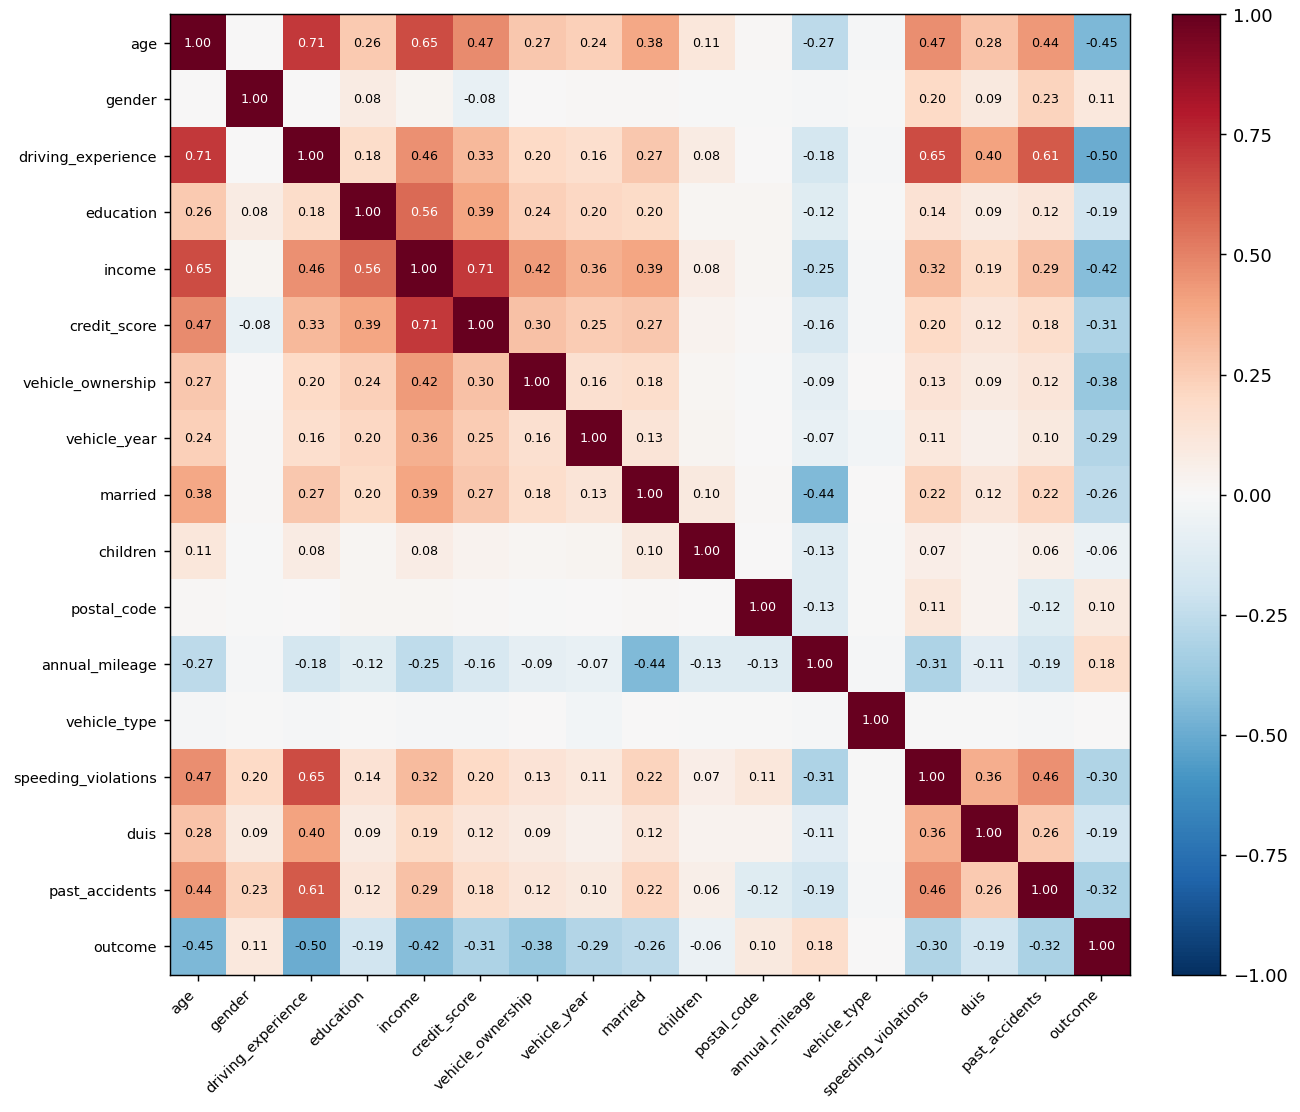
\includegraphics[width=0.82\linewidth]{heatmap.png}
  \caption{Carte des corrélations entre toutes les variables.}
  \label{fig:heatmap}
\end{figure}

\section{Quelles variables annoncent le risque ?}

En se concentrant sur la dernière ligne de la carte, celle qui relie chaque variable au
sinistre, on obtient le classement de la figure~\ref{fig:corr_outcome}. Les variables les
plus liées au risque sont l'expérience de conduite, l'âge, la possession du véhicule, le
nombre d'infractions pour excès de vitesse et le nombre d'accidents passés.

\begin{figure}[H]
  \centering
  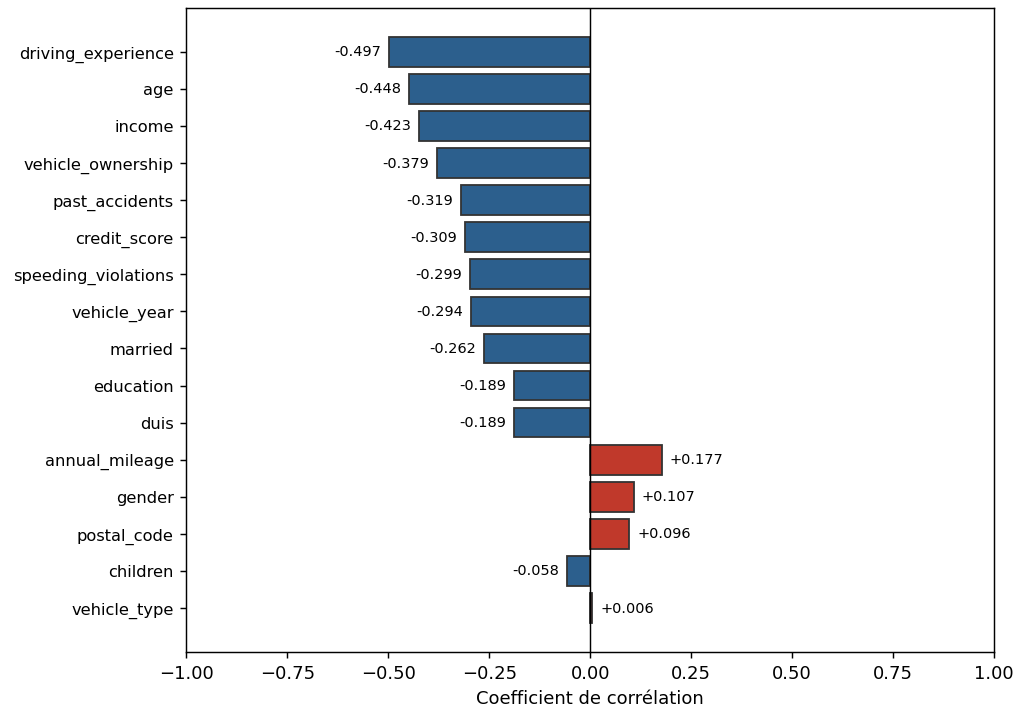
\includegraphics[width=0.85\linewidth]{correlations_outcome.png}
  \caption{Corrélation de chaque variable avec le sinistre.}
  \label{fig:corr_outcome}
\end{figure}

Toutes ces corrélations sont négatives, ce qui se lit très naturellement. Plus
d'expérience, un âge plus avancé ou le fait de posséder son véhicule font \emph{diminuer}
le risque de sinistre. On note enfin que certaines variables d'entrée sont fortement
liées entre elles, par exemple l'âge et l'expérience de conduite, ce qui n'a rien
d'étonnant. Ce phénomène, appelé \textbf{multicolinéarité}, signifie que ces variables
disent en partie la même chose ; le modèle devra répartir entre elles une information
qu'elles se partagent, ce qui explique que leurs poids respectifs puissent paraître plus
modestes qu'attendu.

% ══════════════════════════════════════════════════════════════════════════════
\chapter{Apprendre à partir des données}
% ══════════════════════════════════════════════════════════════════════════════

\section{Pourquoi séparer l'apprentissage de l'évaluation ?}

Voici sans doute le principe le plus important de tout l'apprentissage automatique. Si
l'on entraîne un modèle puis qu'on le juge sur les mêmes données, on se trompe soi-même.
Le modèle pourrait n'avoir fait que \emph{retenir par cœur} les exemples vus, sans rien
comprendre de généralisable. Il obtiendrait alors un excellent score sur ces exemples,
mais s'effondrerait face à des conducteurs nouveaux. Ce travers porte un nom, le
\textbf{surapprentissage}, où le modèle colle tellement aux données d'entraînement qu'il en
perd sa capacité à généraliser.

\begin{figure}[H]
  \centering
  \begin{tikzpicture}[font=\small]
    % barre complète
    \draw[fill=bleudoux!18, draw=bleudoux, line width=0.6pt] (0,0) rectangle (8,1);
    \draw[fill=orangedoux!28, draw=orangedoux, line width=0.6pt] (8,0) rectangle (10,1);
    \draw[line width=0.9pt] (8,-0.1) -- (8,1.1);
    \node at (4,0.5) {\textbf{Apprentissage} — 80\,\%};
    \node at (9,0.5) {\textbf{Test} — 20\,\%};
    \node[below, align=center, text=bleudoux] at (4,-0.2) {8\,000 conducteurs\\{\footnotesize le modèle apprend ici}};
    \node[below, align=center, text=orangedoux!90!black] at (9,-0.2) {2\,000 conducteurs\\{\footnotesize jamais vus à l'entraînement}};
    \node[above] at (5,1.25) {\footnotesize Jeu de données complet — 10\,000 conducteurs};
  \end{tikzpicture}
  \caption{La séparation apprentissage / test.}
  \label{fig:split}
\end{figure}

La parade est simple et illustrée par la figure~\ref{fig:split}. On met de côté une
partie des données, le \textbf{jeu de test}, qu'on ne montrera jamais au modèle pendant
son apprentissage. Le modèle apprend sur le reste, le \textbf{jeu d'apprentissage}, puis
on le juge sur ce jeu de test mis de côté. C'est la seule façon honnête de savoir
s'il a vraiment appris ou seulement récité. On a retenu une répartition classique
de 80~\% pour apprendre et 20~\% pour évaluer, soit huit mille conducteurs d'un côté et
deux mille de l'autre.
\newline
\newline
Une précaution supplémentaire est nécessaire à cause du déséquilibre des classes évoqué
en introduction. Si la séparation se faisait au hasard, on pourrait, par malchance,
concentrer les sinistres d'un côté et les vider de l'autre, faussant l'évaluation. On
emploie donc une découpe dite \textbf{stratifiée}, qui veille à conserver la même
proportion de sinistres dans les deux jeux, fidèle reflet de la réalité.

\section{La régression logistique, un modèle qui raisonne en probabilités}

Pour ce premier modèle, on a retenu la \textbf{régression logistique}, une méthode
de référence pour les problèmes à deux classes. Son principe est simple. Le modèle
commence par calculer un score, en additionnant les variables du conducteur, chacune
multipliée par un \emph{poids} qui dit son importance et son sens. Ce score peut prendre
n'importe quelle valeur, du très négatif au très positif. Or ce que l'on veut, c'est une
\emph{probabilité} de sinistre, donc un nombre entre 0 et 1. C'est là qu'intervient une
fonction en forme de S, la fonction logistique, qui écrase ce score dans l'intervalle
$[0,1]$, comme le montre la figure~\ref{fig:sigmoid}.

\begin{figure}[H]
  \centering
  \begin{tikzpicture}
    \begin{axis}[
      width=0.82\linewidth, height=6.2cm,
      axis lines=middle,
      xlabel={score $z$ calculé à partir du profil}, ylabel={probabilité de sinistre},
      xlabel style={font=\small}, ylabel style={font=\small},
      xmin=-6.5, xmax=6.5, ymin=-0.08, ymax=1.14,
      ytick={0,0.5,1}, xtick={0}, xticklabels={0},
      enlargelimits=false, clip=false]
      \addplot[domain=-6.5:6.5, samples=140, very thick, bleudoux]{1/(1+exp(-x))};
      \addplot[densely dashed, gray, domain=-6.5:6.5, samples=2]{0.5};
      \node[anchor=west, vertdoux!70!black] at (axis cs:-6.2,0.93) {\footnotesize on prédit un sinistre};
      \node[anchor=west, rougedoux] at (axis cs:-6.2,0.10) {\footnotesize on prédit l'absence de sinistre};
      \node[anchor=south, fill=white, inner sep=1pt, gray] at (axis cs:2.4,0.5) {\footnotesize seuil de décision = 0,5};
    \end{axis}
  \end{tikzpicture}
  \caption{La fonction logistique.}
  \label{fig:sigmoid}
\end{figure}

Entraîner ce modèle, c'est chercher les poids qui rendent ses probabilités les plus
fidèles possible à la réalité observée. Il n'existe pas de formule magique donnant la
réponse d'un coup ; l'ordinateur procède par essais successifs, ajustant peu à peu les
poids jusqu'à ce qu'ils ne s'améliorent plus. Au bout du compte, le modèle a appris deux
choses, un poids par variable et un terme constant appelé biais qui règle sa tendance
générale.

\section{Ce que le modèle a retenu}

Une fois entraîné, le modèle reconnaît correctement environ 85~\% des conducteurs de son
jeu d'apprentissage. Surtout, ses poids se lisent comme une explication, présentée à la
figure~\ref{fig:coef}. Un poids négatif (en bleu) pousse vers l'absence de sinistre, un
poids positif (en rouge) vers le sinistre, et plus la barre est longue, plus la variable
pèse.

\begin{figure}[H]
  \centering
  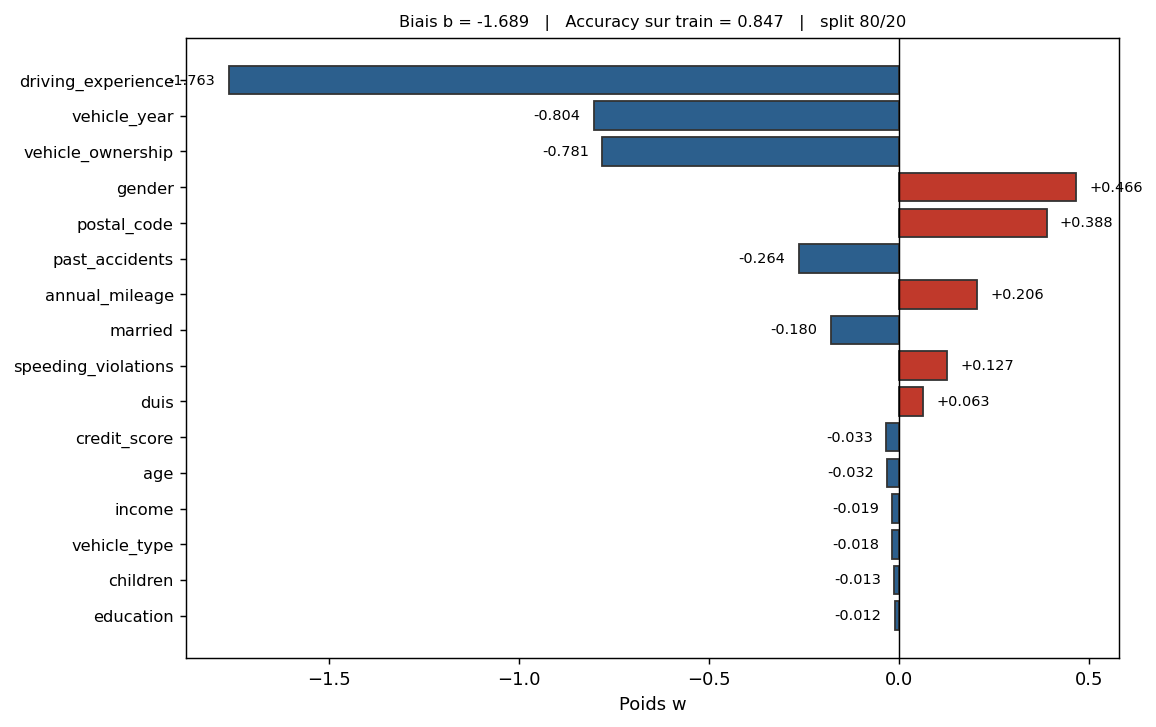
\includegraphics[width=0.9\linewidth]{coefficients.png}
  \caption{Importance et sens de chaque variable.}
  \label{fig:coef}
\end{figure}

Le verdict du modèle rejoint l'intuition et confirme l'analyse des corrélations.
L'expérience de conduite est de très loin le facteur le plus protecteur. Le terme constant
est nettement négatif, ce qui traduit simplement que, dans le doute, le modèle parie sur
l'absence de sinistre, puisque c'est le cas le plus fréquent. On obtient ainsi non
seulement un outil de prédiction, mais aussi une grille de lecture du risque.

% ══════════════════════════════════════════════════════════════════════════════
\chapter{Évaluer honnêtement la qualité du modèle}
% ══════════════════════════════════════════════════════════════════════════════

Disposer d'un modèle ne suffit pas ; encore faut-il savoir ce qu'il vaut. Et bien
évaluer est plus subtil qu'il n'y paraît, surtout lorsque les classes sont déséquilibrées.

\section{La matrice de confusion}

Toutes les erreurs ne se valent pas. Annoncer un sinistre qui n'arrivera pas (une fausse
alerte) et passer à côté d'un vrai sinistre n'ont pas les mêmes conséquences. Pour ne rien
masquer, on dresse la \textbf{matrice de confusion}, qui croise ce que le modèle a prédit
avec ce qui s'est réellement passé, et range les conducteurs dans quatre cases
(figure~\ref{fig:confmat_schema}).

\begin{figure}[H]
  \centering
  \begin{tikzpicture}[font=\small]
    % cellules
    \fill[vertdoux!18] (0,2) rectangle (4,4);
    \fill[rougedoux!15] (4,2) rectangle (8,4);
    \fill[rougedoux!15] (0,0) rectangle (4,2);
    \fill[vertdoux!18] (4,0) rectangle (8,2);
    \draw[line width=0.6pt, xstep=4, ystep=2] (0,0) grid (8,4);
    \draw[line width=0.6pt] (0,0) rectangle (8,4);
    % contenu des cellules
    \node[align=center] at (2,3) {\textbf{Vrai positif}\\{\footnotesize sinistre prédit\\et survenu}};
    \node[align=center] at (6,3) {\textbf{Faux négatif}\\{\footnotesize sinistre raté}\\{\scriptsize(le plus grave)}};
    \node[align=center] at (2,1) {\textbf{Faux positif}\\{\footnotesize fausse alerte}};
    \node[align=center] at (6,1) {\textbf{Vrai négatif}\\{\footnotesize absence correctement\\prédite}};
    % en-têtes colonnes
    \node[above] at (2,4.15) {\textbf{Prédit sinistre}};
    \node[above] at (6,4.15) {\textbf{Prédit absence}};
    % en-têtes lignes
    \node[rotate=90, anchor=south] at (-0.25,3) {\textbf{Réel sinistre}};
    \node[rotate=90, anchor=south] at (-0.25,1) {\textbf{Réel absence}};
  \end{tikzpicture}
  \caption{Les quatre cases de la matrice de confusion.}
  \label{fig:confmat_schema}
\end{figure}

Appliquée au jeu de test, cette matrice donne les chiffres de la
figure~\ref{fig:confusion}. Le modèle identifie correctement la grande majorité des cas,
avec un nombre modéré de fausses alertes et de sinistres manqués.

\begin{figure}[H]
  \centering
  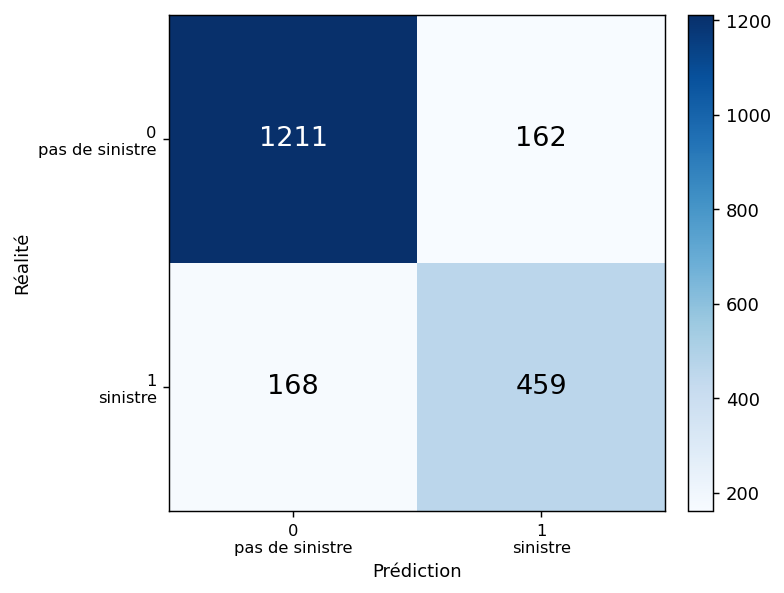
\includegraphics[width=0.58\linewidth]{matrice_confusion.png}
  \caption{Matrice de confusion sur les 2\,000 conducteurs de test.}
  \label{fig:confusion}
\end{figure}

\section{Au-delà du simple taux de bonnes réponses}

La mesure la plus naturelle de la performance est l'\textbf{exactitude} (souvent appelée
\emph{accuracy}), c'est-à-dire la part de conducteurs correctement classés, toutes
catégories confondues. Elle est utile, mais traîtresse lorsque les classes sont déséquilibrées. Dans
le cas présent, un modèle paresseux qui ne prédirait jamais de sinistre pour personne
atteindrait déjà environ 69~\% d'exactitude, sans rien avoir compris. Se contenter de
cette mesure serait donc trompeur.
\newline
\newline
C'est pourquoi on regarde deux autres indicateurs, qui éclairent des aspects
complémentaires et qu'il faut bien distinguer :

\begin{itemize}
  \item La \textbf{précision} demande si, lorsque le modèle annonce un
        sinistre, il a raison. Une précision élevée signifie peu de fausses alertes.
  \item Le \textbf{rappel}, lui, mesure combien des vrais
        sinistres le modèle retrouve effectivement. Un rappel élevé signifie peu de
        sinistres manqués.
\end{itemize}

\encadre{Précision et rappel, deux exigences en tension}{La différence entre les deux est
au cœur de l'évaluation. Un modèle qui ne crierait au sinistre que lorsqu'il en est
absolument certain serait très précis mais raterait beaucoup de cas (rappel faible). À
l'inverse, un modèle qui crierait au sinistre à la moindre alerte attraperait tout le
monde (rappel élevé) au prix d'innombrables fausses alertes (précision faible). Le
\textbf{F1-score} réconcilie les deux en une seule note, en récompensant les modèles qui
trouvent un bon équilibre.}

Sur le jeu de test, précision et rappel se tiennent tous deux autour de 0,73, et sont
quasiment égaux. Cet équilibre est une bonne nouvelle, car compte tenu du déséquilibre des
classes, le modèle ne sacrifie ni la chasse aux sinistres ni la limitation des fausses
alertes. La figure~\ref{fig:metriques} récapitule ces indicateurs.

\begin{figure}[H]
  \centering
  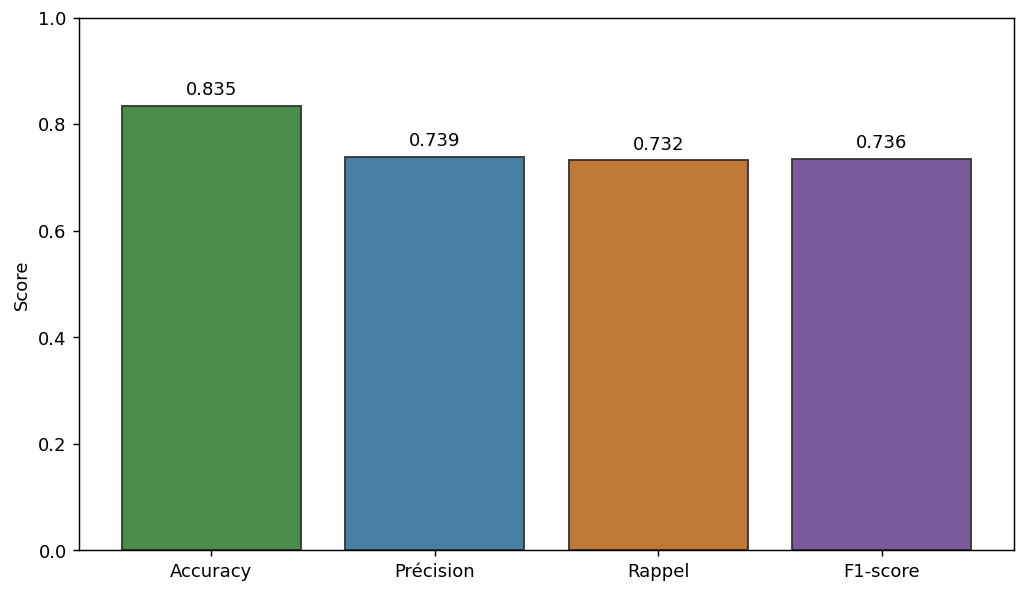
\includegraphics[width=0.72\linewidth]{metriques.png}
  \caption{Les indicateurs de performance sur le jeu de test.}
  \label{fig:metriques}
\end{figure}

\section{La validation croisée, parce qu'un seul essai ne prouve rien}

Tous ces chiffres reposent sur une unique découpe des données. Mais si cette découpe avait
été chanceuse ? Pour s'assurer que la performance n'est pas un coup de dé, on emploie la
\textbf{validation croisée}. L'idée, illustrée à la figure~\ref{fig:kfold}, est de
découper le jeu d'apprentissage en cinq parts égales, puis de répéter cinq fois
l'expérience. À chaque tour, une part différente sert de mini-jeu de test pendant que les
quatre autres servent à apprendre. On obtient ainsi cinq évaluations indépendantes, dont
on regarde la moyenne et la dispersion.

\begin{figure}[H]
  \centering
  \resizebox{0.92\linewidth}{!}{%
  \begin{tikzpicture}[font=\footnotesize]
    \foreach \r in {1,...,5}{
      % cinq blocs d'entraînement
      \foreach \c in {1,...,5}{
        \fill[bleudoux!20, draw=white, line width=1pt]
          ({(\c-1)*2.1},{-\r*0.95}) rectangle ({(\c-1)*2.1+2},{-\r*0.95+0.72});
      }
      % le bloc de validation pour cet essai (colonne = numéro d'essai)
      \fill[orangedoux!55, draw=white, line width=1pt]
        ({(\r-1)*2.1},{-\r*0.95}) rectangle ({(\r-1)*2.1+2},{-\r*0.95+0.72});
      \node[left] at (-0.3,{-\r*0.95+0.36}) {Essai \r};
    }
    % légende
    \fill[bleudoux!20] (0,-5.7) rectangle (0.5,-5.35);
    \node[right] at (0.55,-5.52) {blocs d'entraînement};
    \fill[orangedoux!55] (4.6,-5.7) rectangle (5.1,-5.35);
    \node[right] at (5.15,-5.52) {bloc de validation};
  \end{tikzpicture}}
  \caption{La validation croisée à cinq plis.}
  \label{fig:kfold}
\end{figure}

Le résultat est rassurant, les cinq scores se regroupant autour de 0,846 avec une
dispersion très faible (figure~\ref{fig:cv}). Cette stabilité confirme que la performance
du modèle ne tient pas à une découpe particulière, mais reflète une réelle capacité à
généraliser. La différence entre l'évaluation sur une seule découpe et la validation
croisée est précisément là, la première donnant une photographie, la seconde une moyenne
de plusieurs photographies, donc une mesure plus fiable.

\begin{figure}[H]
  \centering
  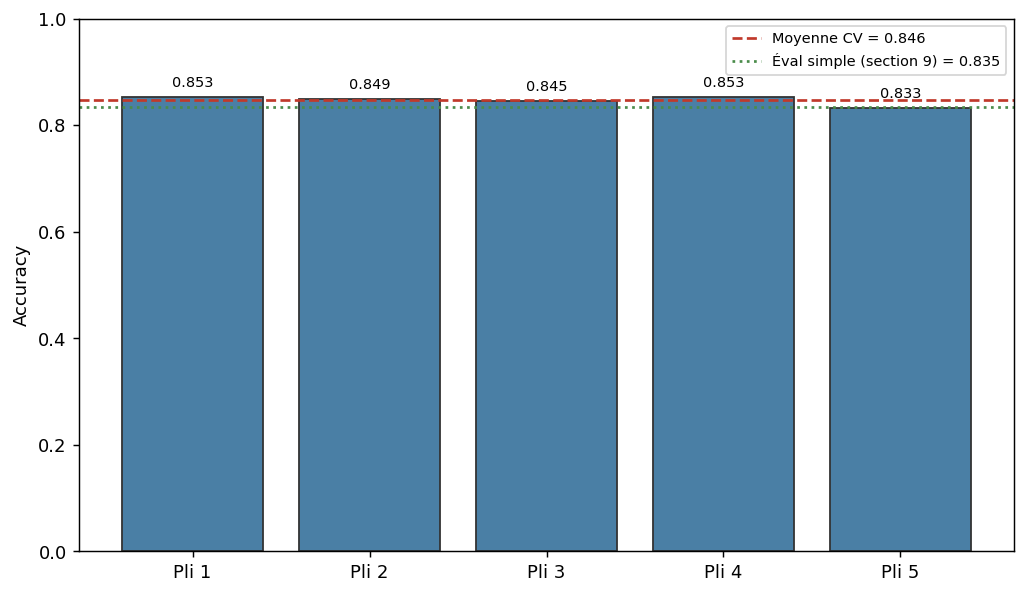
\includegraphics[width=0.78\linewidth]{scores_cv.png}
  \caption{Les cinq scores de la validation croisée.}
  \label{fig:cv}
\end{figure}

% ══════════════════════════════════════════════════════════════════════════════
\chapter{Comparer les algorithmes et retenir le meilleur}
% ══════════════════════════════════════════════════════════════════════════════

La régression logistique donne de bons résultats, mais rien ne dit qu'elle soit le
meilleur choix. Pour en avoir le cœur net, on la met en concurrence avec d'autres familles
d'algorithmes, dans des conditions strictement identiques.

\section{Trois façons différentes d'apprendre}

Les algorithmes comparés reposent sur des idées très différentes, qu'il est utile de
distinguer car leur diversité éclaire les résultats :

\begin{itemize}
  \item La \textbf{régression logistique} cherche une frontière régulière entre les deux
        classes et raisonne en probabilités, comme on l'a vu.
  \item Le \textbf{perceptron} cherche lui aussi une frontière linéaire, mais de façon
        plus rudimentaire, tranchant de manière nette, sans nuance de probabilité, ce
        qui le rend plus sensible aux cas difficiles.
  \item Les \textbf{$k$ plus proches voisins} adoptent une stratégie radicalement
        différente, illustrée par la figure~\ref{fig:knn}. Pour classer un nouveau
        conducteur, ils regardent les profils les plus ressemblants déjà connus et leur
        font voter. Ils n'apprennent pas de règle générale, ils comparent.
\end{itemize}

\begin{figure}[H]
  \centering
  \begin{tikzpicture}[font=\footnotesize]
    \draw[->, gray] (-0.2,-0.2) -- (5.2,-0.2);
    \draw[->, gray] (-0.2,-0.2) -- (-0.2,4.2);
    % classe 0 (vert)
    \foreach \p in {(0.6,0.7),(1.0,1.6),(0.4,2.3),(1.4,0.6),(0.9,3.1),(1.7,2.6)}
      \fill[vertdoux] \p circle (2.4pt);
    % classe 1 (rouge)
    \foreach \p in {(3.8,3.4),(4.2,2.4),(3.2,2.0),(4.5,3.6),(3.6,1.3),(2.9,3.4)}
      \fill[rougedoux] \p circle (2.4pt);
    % point à classer
    \node[star, star points=5, star point ratio=2.3, fill=orangedoux, draw=black, inner sep=1.6pt] (q) at (2.5,2.4) {};
    % cercle des voisins
    \draw[densely dashed, gray] (2.5,2.4) circle (1.15cm);
    \node[anchor=west] at (2.6,0.5) {\textcolor{orangedoux!90!black}{$\star$} = conducteur à classer};
    \node[anchor=west] at (2.6,0.05) {cercle = ses plus proches voisins};
  \end{tikzpicture}
  \caption{Le principe des $k$ plus proches voisins.}
  \label{fig:knn}
\end{figure}

\section{Le verdict de la comparaison}

Tous ces modèles sont évalués avec la même validation croisée à cinq plis, pour que la
comparaison soit équitable. Pour les plus proches voisins, on essaie en outre plusieurs
valeurs du nombre de voisins consultés, car c'est leur réglage déterminant. La
figure~\ref{fig:comparaison} et le tableau~\ref{tab:comparaison} rassemblent les
résultats.

\begin{figure}[H]
  \centering
  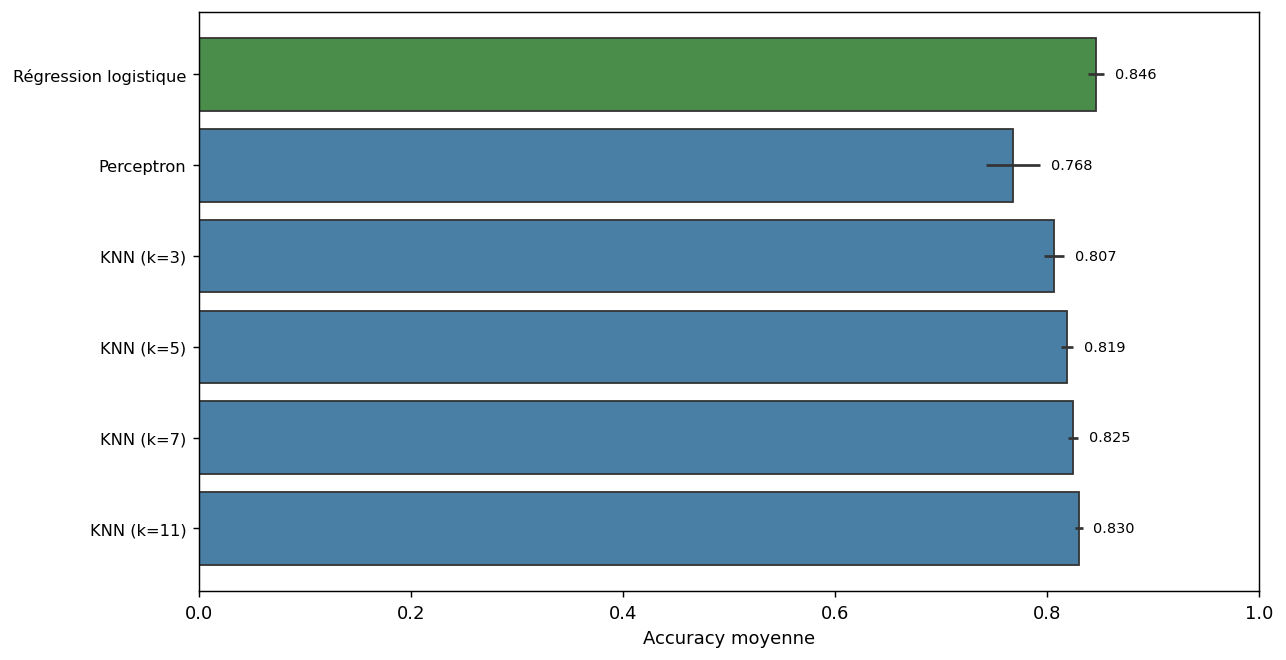
\includegraphics[width=0.88\linewidth]{comparaison.png}
  \caption{Performance moyenne de chaque algorithme.}
  \label{fig:comparaison}
\end{figure}

\begin{table}[H]
  \centering
  \begin{tabular}{lc}
    \toprule
    \textbf{Algorithme} & \textbf{Exactitude moyenne (validation croisée)} \\
    \midrule
    Régression logistique & \textbf{0,846} \\
    $k$ plus proches voisins ($k=11$) & 0,830 \\
    $k$ plus proches voisins ($k=7$) & 0,825 \\
    $k$ plus proches voisins ($k=5$) & 0,819 \\
    $k$ plus proches voisins ($k=3$) & 0,807 \\
    Perceptron & 0,768 \\
    \bottomrule
  \end{tabular}
  \caption{Classement des algorithmes.}
  \label{tab:comparaison}
\end{table}

Deux enseignements se dégagent. D'abord, pour les plus proches voisins, consulter
davantage de voisins améliore et stabilise le résultat, car un nombre trop petit rend la
décision sensible au moindre cas particulier. Ensuite, et surtout, aucun concurrent ne
parvient à dépasser la régression logistique. Le perceptron, en particulier, ferme la
marche et se montre le plus instable, ce qui s'explique par sa façon trop tranchée de
décider. La conclusion est sans appel. Pour ce problème, la régression logistique offre
le meilleur compromis entre justesse, stabilité et lisibilité.

\section{Conserver le modèle pour le réutiliser}

Une fois le meilleur modèle identifié, il serait dommage de devoir le réentraîner à chaque
usage. On le \textbf{sauvegarde} donc sur le disque, dans un fichier, d'où on pourra le
ressortir instantanément. Pour s'assurer que cette sauvegarde est fidèle, on procède à une
vérification simple. On recharge le modèle enregistré et l'on compare ses prédictions à
celles du modèle d'origine sur quelques conducteurs. Les réponses sont rigoureusement
identiques, ce qui confirme que le modèle conservé est bien le même que celui que l'on a
entraîné, prêt à être déployé.

% ══════════════════════════════════════════════════════════════════════════════
\SpecialSection{Conclusion}
% ══════════════════════════════════════════════════════════════════════════════

Ce projet aura déroulé, d'un bout à l'autre, la chaîne complète d'une étude de données,
des conducteurs bruts et imparfaits du fichier de départ jusqu'à un modèle capable de
prédire le risque de sinistre et conservé pour un usage futur. Le résultat est solide,
puisque le modèle reconnaît correctement plus de huit conducteurs sur dix, avec une stabilité
confirmée par la validation croisée, et il l'emporte sur les autres algorithmes essayés.
\newline
\newline
Mais c'est moins le chiffre final que la \emph{démarche} qui constitue le véritable
acquis. Trois idées nous semblent mériter d'être retenues. La première est qu'un modèle ne
vaut que ce que valent ses données, et que l'essentiel du travail, le plus délicat, réside
dans la préparation, bien avant l'entraînement proprement dit. La deuxième est qu'on ne
doit jamais appliquer une recette toute faite sans réfléchir à la nature de ce que l'on
manipule ; la même opération peut soigner une variable et en détruire une autre. La
troisième, enfin, est qu'évaluer un modèle est un art en soi, car un bon score sur les
données d'entraînement ne prouve rien, et seule une évaluation honnête, sur des données
jamais vues et répétée plusieurs fois, permet de juger sa vraie valeur.
\newline
\newline
Au fond, ce projet nous aura appris qu'en science des données, la rigueur de la méthode
compte davantage que la sophistication de l'outil. Un modèle simple, mais nourri de
données soigneusement préparées et évalué sans complaisance, l'emporte presque toujours
sur un modèle compliqué construit sur des bases fragiles.

\end{document}
